\documentclass[a4paper, 11pt]{article}
\usepackage[english]{babel}
\usepackage{mathpazo}
\usepackage{amsmath}	
\usepackage{amssymb}	
\usepackage{mathrsfs}
\usepackage{amsthm}
\usepackage{subfig}
\usepackage{placeins}
\usepackage{stmaryrd}
\usepackage{minted}
\usepackage{tikz}
\usepackage[top=2cm, bottom=2cm, right=2cm, left=2cm]{geometry}
\usepackage[pdfencoding=auto, hidelinks]{hyperref}
\usepackage{bookmark}
\usepackage{xparse}

\newcommand{\RR}{\mathbb{R}}
\newcommand{\NN}{\mathbb{N}}
\newcommand{\floor}[1]{{\left\lfloor #1 \right\rfloor}}

\DeclareDocumentCommand{\todo}{g}{
	\textcolor{red}{{\Large TODO}}
	\IfNoValueF{#1}{
		\textcolor{red}{{\Large: #1}}
	}
}

\DeclareDocumentCommand{\wtf}{g}{
	\textcolor{red}{{\Large WTF}}
	\IfNoValueF{#1}{
		\textcolor{red}{{\Large: #1}}
	}
}

\title{Simulated annealing algorithm for graph coloring}
\author{
	Marc \textsc{Chevalier}\\
	Yannick \textsc{Grimault}\\
	George \textsc{Zakhour}
}

\begin{document}
\maketitle

\section{Choice of \texorpdfstring{$\beta$}{β}}


To choose $\beta$ among all possible functions, our first approach was to use a polynomial and, using bandit, make the coefficient converge to an optimal polynomial for the given degree. We hopped that the coefficient represent a well known power series and retrieve a good function. But several problem appears. First, this problem is not a priori convex. Thus, the best we can do is to find a local minimum (or use simulated annealing but it makes the problem recursive). However, this method is still useful to find local minima which can be good idea or to test if a candidate function is a minimum: in this case, it is a fixpoint.

Starting from the initial polynomial $\sum\limits_{i=0}^n X^i$, the algorithm converge quickly but to a very close polynomial. This is not a good news a priori since $\sum\limits_{i=0} x^i = \frac{1}{1-x}$ with a radius of convergence of 1. This is a bad news since the temperature is affine decreasing, thus reach 0 in finite time, ie. $\beta$ diverges in finite time.

\bigskip

Functions of the form $x\mapsto k\exp(ax)$ are pretty interesting for different reasons. First (but not very convincing) the inverse is a function of the form $x\mapsto k^{-1}\exp(-ax)$ which is the kind of functions we found when we let an object spontaneously cool. Moreover, it is this kind of function we found in the literature (eg.~\cite{chams1987some}). Finally, these functions are fixpoints of our bandit. So, it seems reasonable to use a function like
\[
	\begin{aligned}
		\beta : \NN &\to \RR\\
		n &\mapsto \beta_0\exp\left(a\floor{\frac{n}{\tau}}\right)
	\end{aligned}
\]
This function is constant on any interval $\llbracket k\tau; (k+1)\tau -1\rrbracket$ for all non negative integer $k$ and $\forall k\in\NN, \exp(-a)\beta(k\tau) = \beta((k+1)\tau)$. Thus, in the following, we will adapt only two parameters: $a$ and $\tau$ (which impact strongly the quality of the result~\cite{chams1987some}).

To find these parameters we have used a modified version of the bandit. \todo{results}

The bandit as we did it find only constant parameters. To follow the idea of the paper, hoping we improve the quality of the approximation, we allow $\tau$ to depend on the previous $\beta$, thus $\beta(n)$ for $n>0$ depends on $n$ and $\beta(n-1)$. In the simulations, we take $\beta_0 = {\lvert V\rvert}^{-\frac{1}{2}}$, $\tau = \floor{\exp(2\beta(n-1))+\frac{1}{2}}$ (nearest integer) and $a = -\ln(0.93)$.

\section{Comments on the implementation}

The graph is stored as the adjacency lists. They are efficient for storing and allow direct access of the neighbours.

The colouring is compute by another class. In an optimizing aim, the Hamiltonian is simply updated and not recomputed at each step. For the sake of flexibility, the parameter $\beta$ is a function. In this way, we allow any pattern for beta without modifying this class.

We used \texttt{matplotlib} to plot.

The implementation of the \textsc{Metropolis} algorithm can keep the minimum energy and the colouring achieving it. Thus, we can run the algorithm as long as we want, even if the energy increase at the end, we have access to the best found colouring.

We see the implementation is pretty fast since we can compute $10^5$ iterations of \textsc{Metropolis} algorithm on a graph with 1000 edges in less than one second.

For some heavy computation (such as the question 4), we used multiprocessing in order to reduce the computation time.

\section{Question 3}

\begin{figure}[!ht]
	\centering
	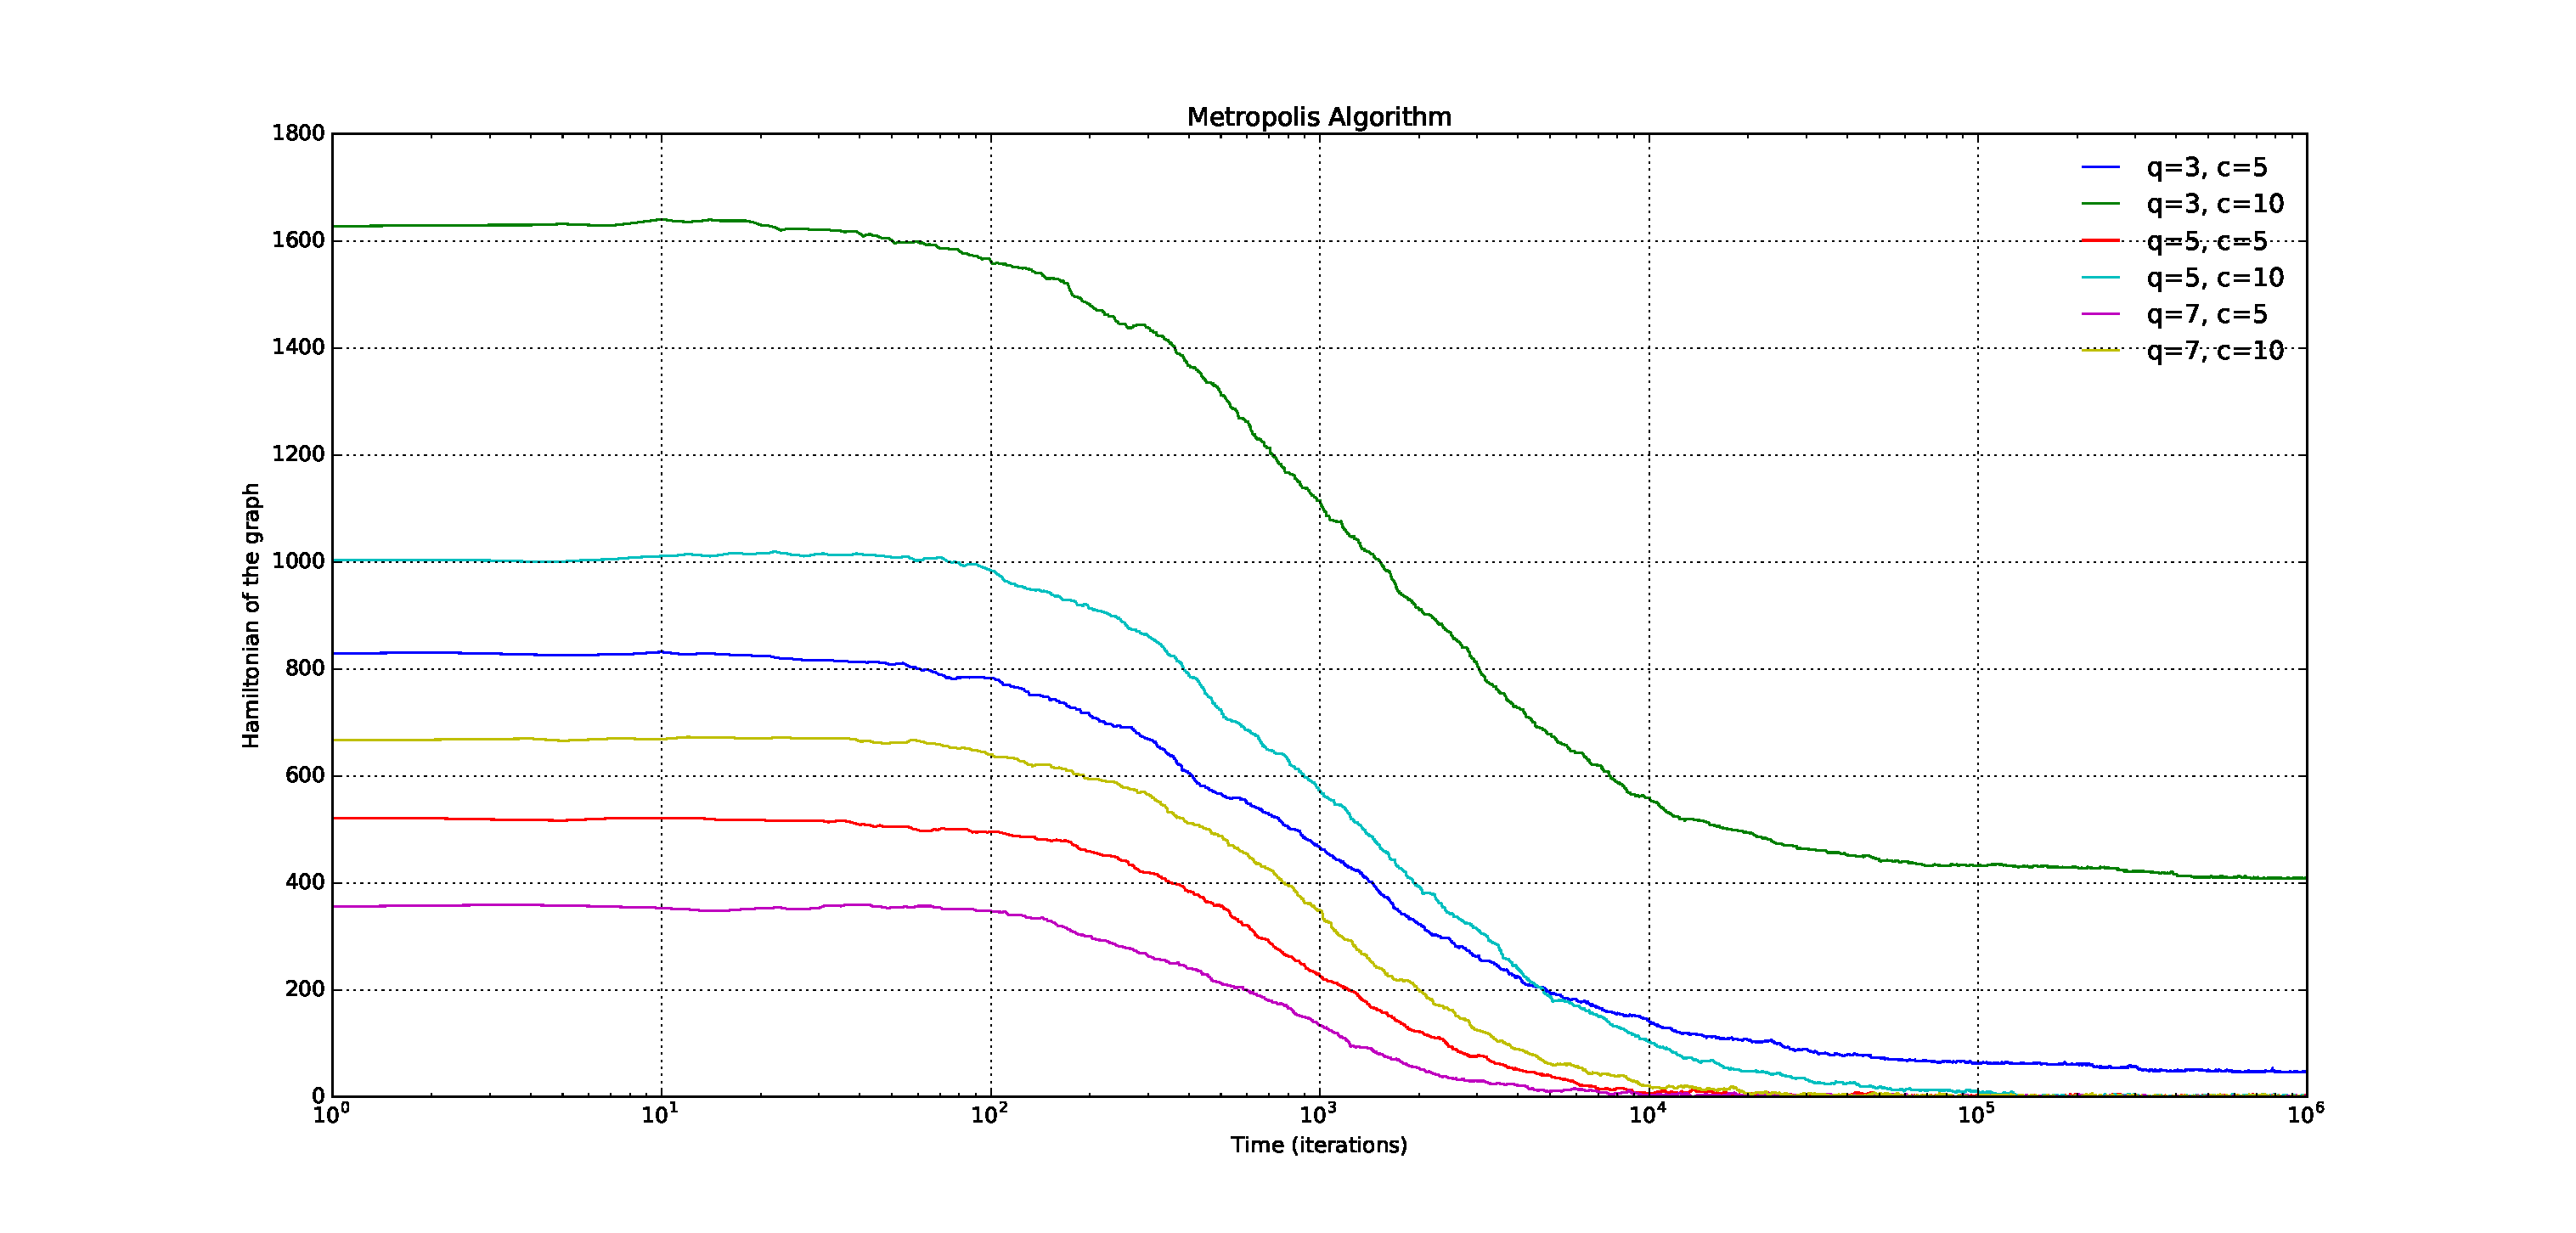
\includegraphics[width=\textwidth]{figures/q3}
	\caption{Hamiltonian as a function of time on an \textsc{Erd\H{o}s-Renyi} graph with 1000 vertices}
\end{figure}

We tried the decade $[10^6; 10^7]$ but nothing happen here (except complains of a suffering RAM).

We see that the energy drops at least to a third. In some case, a perfect colouring is found.

\FloatBarrier

\section{Question 4}

\begin{figure}[!ht]
	\centering
	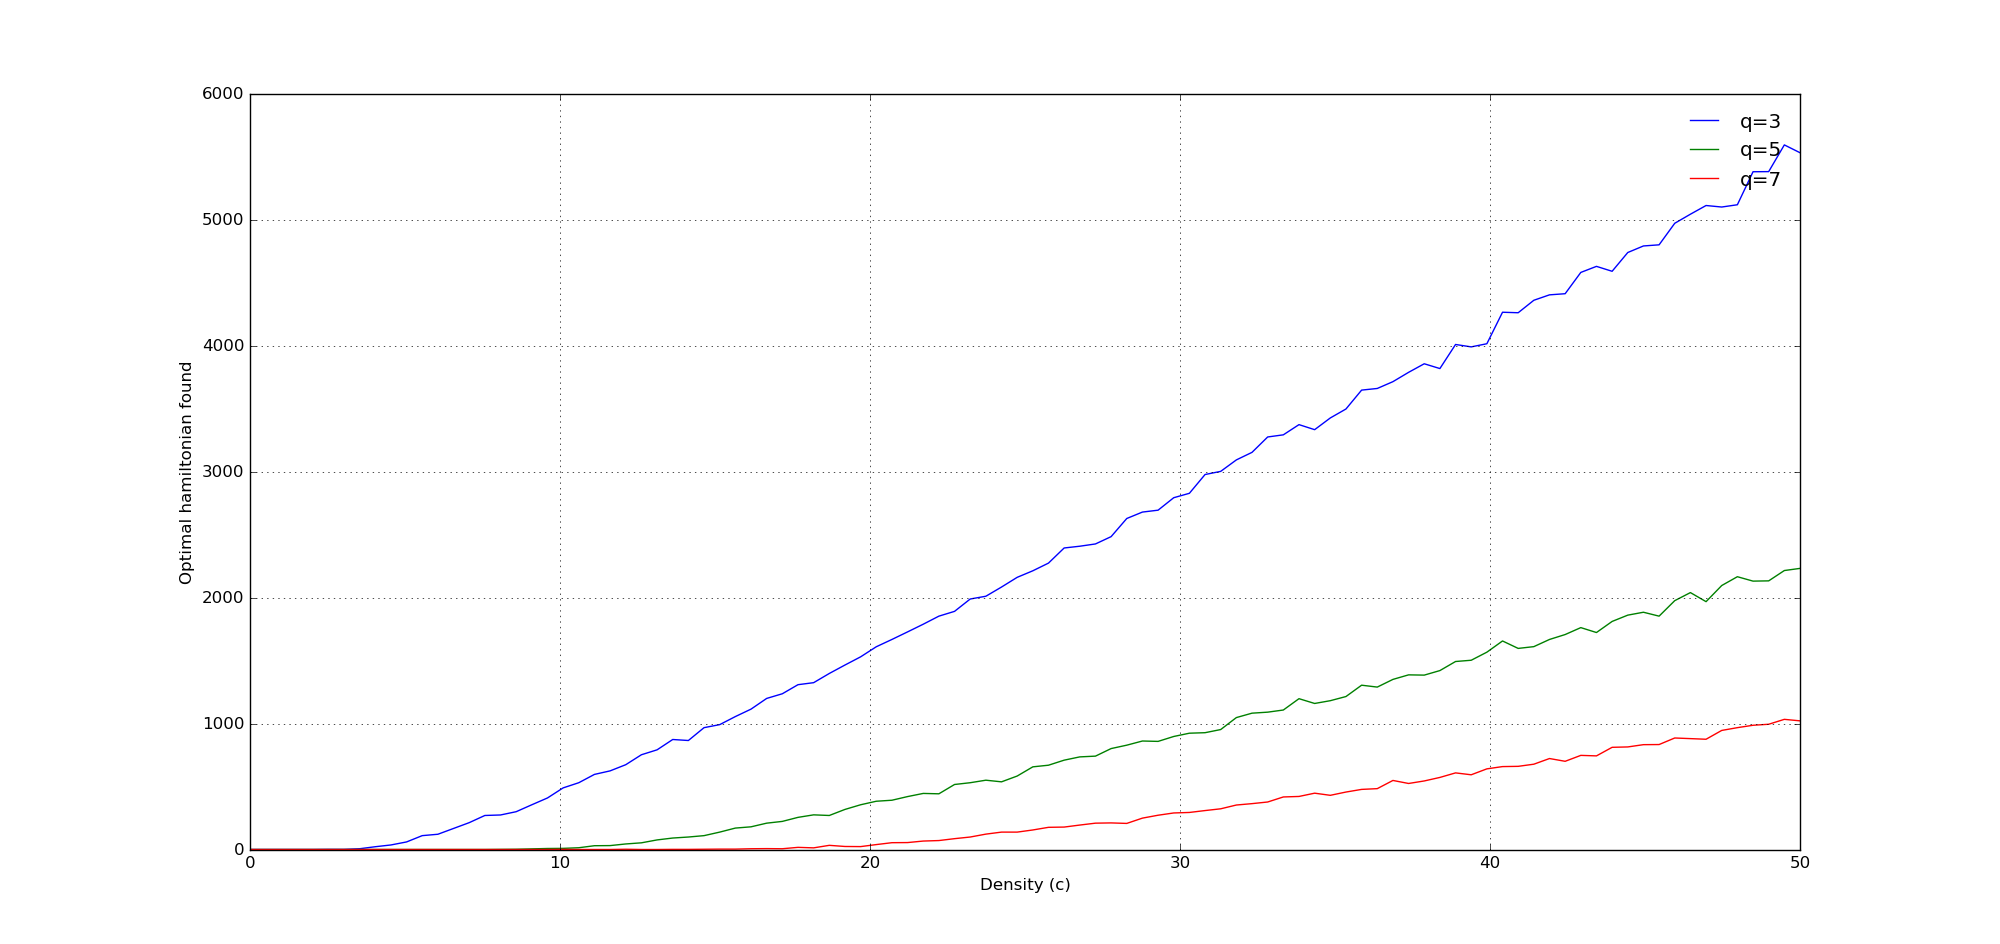
\includegraphics[width=\textwidth]{figures/q4}
	\caption{Minimum Hamiltonian as a function of the connectivity on \textsc{Erd\H{o}s-Renyi} graphs with 1000 vertices and $10^5$ iterations}
\end{figure}

As expected, when the connectivity increase the Hamiltonian increase as well. We see that we can better colour graph when more colours are allowed. This is pretty obvious, too.

The curves seems roughly affine but the slope is lower with more colours.

For $q=3$, the energy increase by about 1500 for 5000 new edges. But only 700 when $q=5$ and about 200 when $q=7$.

\todo{More comments?}

\FloatBarrier

\bibliographystyle{alpha}
\bibliography{report}

\end{document}